\section{Motivation}
\label{sec:motiv}
%
This section provides the motivation that underlies the design decisions of \neupims.
%
First, we identify problems of the existing GPU-based LLM inference serving systems, which motivates the NPU-PIM heterogeneous approach. 
%
Then, we will discuss the limitations of na\"ive NPU-PIM integration approach, defining the target research challenges of this work.

\subsection{GPU-based LLM Inference Serving}
\label{sec:gpu-analysis}

%
%
%
%
Particularly for LLMs, as they require a lot of memory, it is a common practice to deploy them on a cluster of multiple GPUs~\cite{deepspeed, nvidia_triton, tensorrt, onnxruntime, hugging-face}, leveraging pipeline parallelism~\cite{pipedream, gpipe} and/or tensor parallelism~\cite{megatronlm, alpa}.
%

\begin{figure}[t]
        \centering
        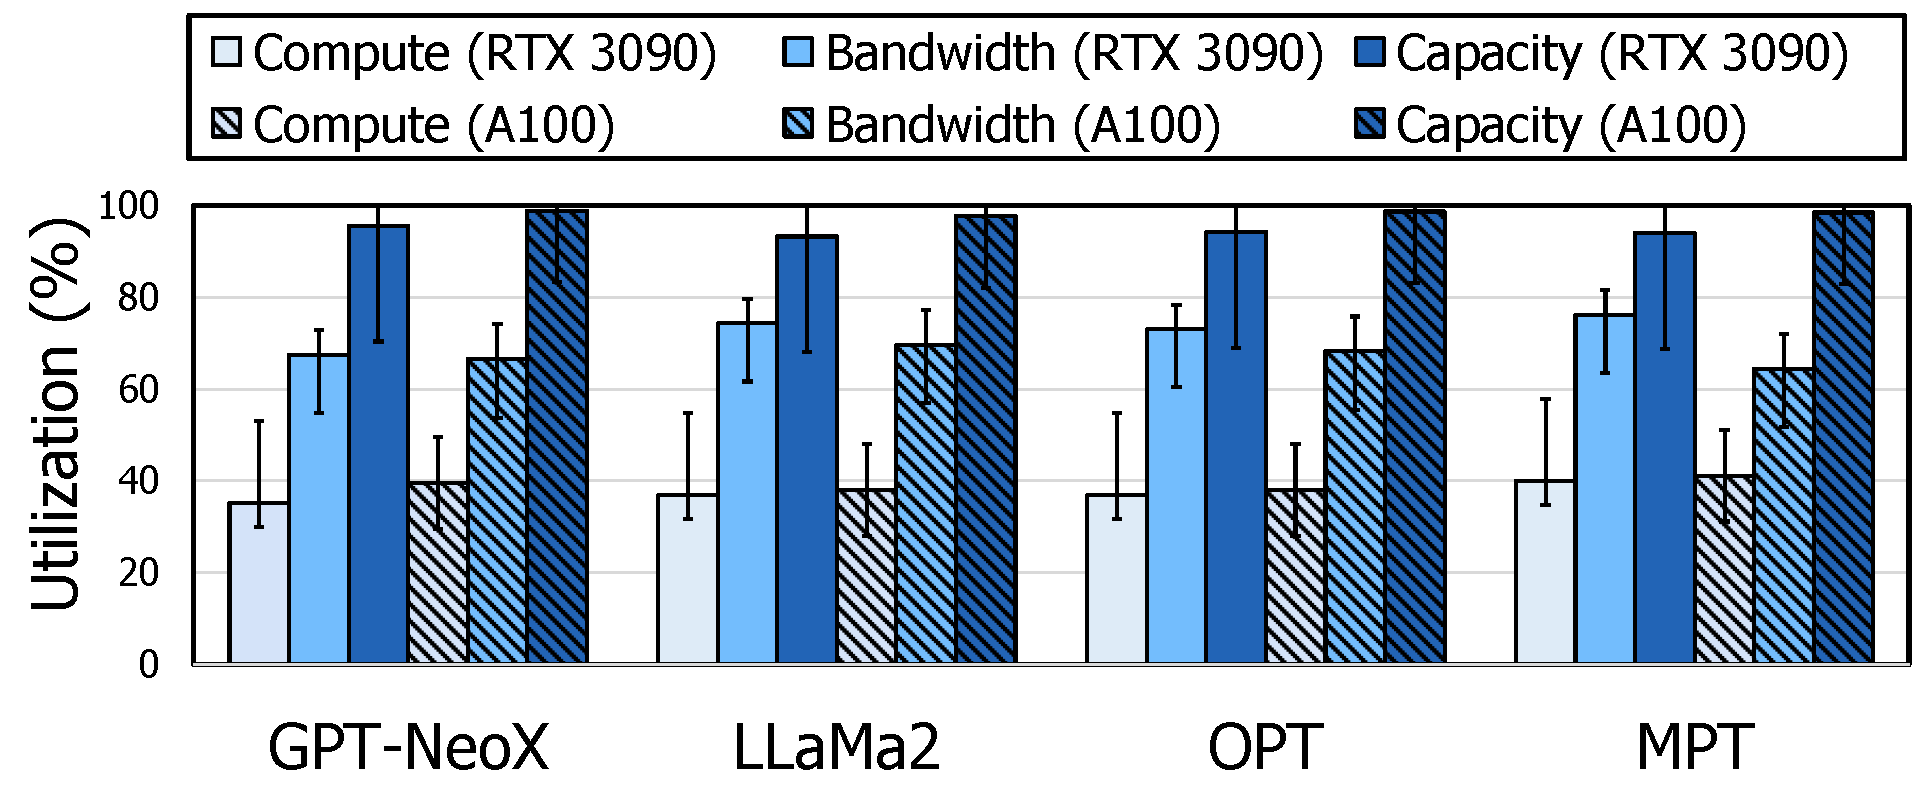
\includegraphics[width=0.9\linewidth]{figure/motiv-gpu-util.pdf}
        \vspace{-2ex}
        \caption{GPU resource utilization for four different LLMs. }
        \vspace{-3ex}
        \label{fig:gpu-utilization}
\end{figure}

\niparagraph{Under-utilization of the GPU system.}
%
We analyze a GPU-equipped baseline system to understand the utilization of compute, memory, and bandwidth for LLM inference.
%
We compare systems with NVIDIA GeForce RTX 3090 24GB and NVIDIA A100 40GB, running four different LLM models: GPT-NeoX, LLaMa2, OPT, and MPT. 
%
Figure~\ref{fig:gpu-utilization} presents the utilization results along with the layer-wise variations as error bars. 
%
The figure illustrates that the capacity utilization closely approaches 100\% despite the inherent imperfections in the parallelization schemes.
%
This observation is intuitive as the number of GPUs used is determined based on the capacity constraints.
%
However, the utilization of computational resources is consistently lower than 40\%, which shows the cost-ineffectiveness of GPU-based LLM inference systems. 
%
This under-utilization is attributed to insufficient bandwidth, despite A100s being equipped with HBM, providing an aggregate of 1,555 GB/s.
%
Unfortunately, this imbalance is inevitable as long as serial dependencies between GEMMs and GEMVs persist. 
%

\begin{figure}[t]
        \centering
        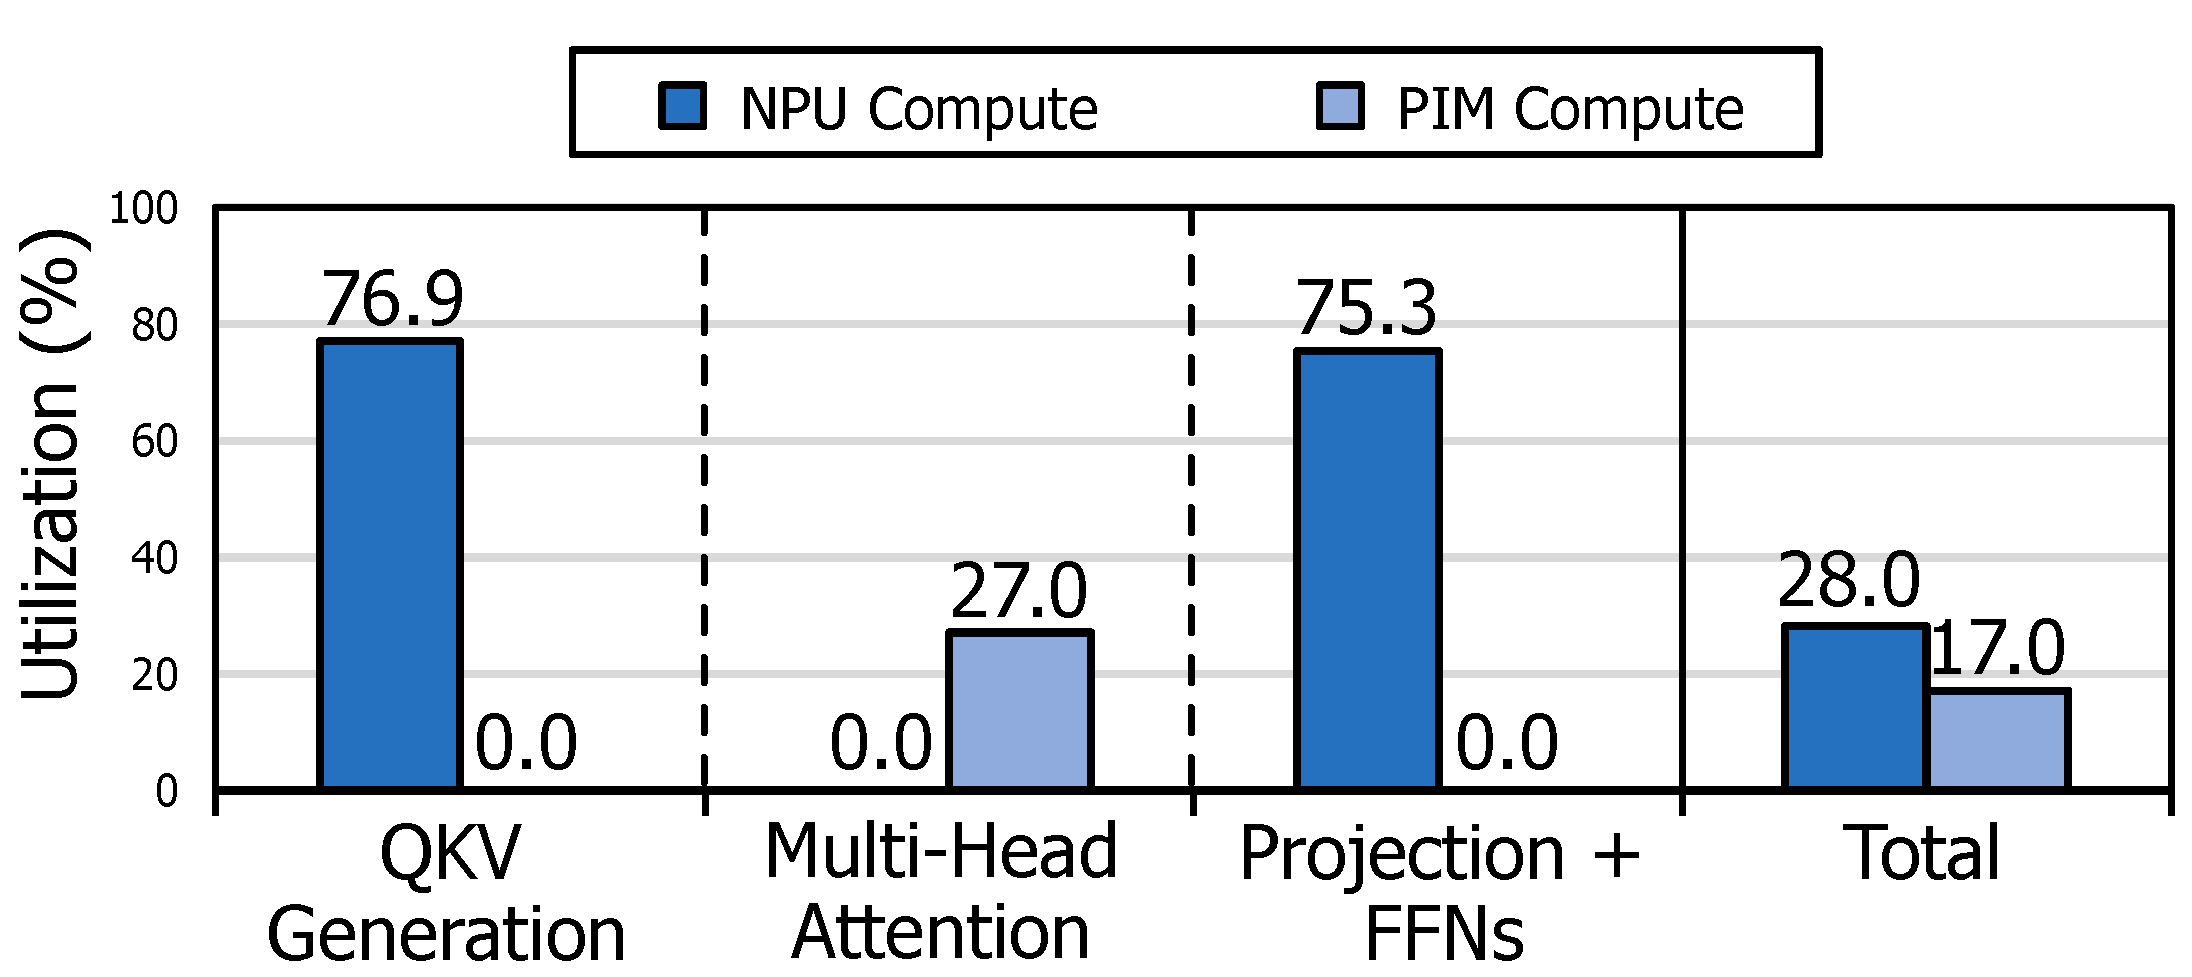
\includegraphics[width=0.9\linewidth]{figure/motiv-mha-block-npu-pim-breakdown-new-svg.pdf}
        \vspace{-2ex}
        \caption{NPU-PIM resource utilization for decoder block.}
        \vspace{-3ex}
        \label{fig:npupim-utilization}
\end{figure}


\begin{figure*}[t]
        \centering
        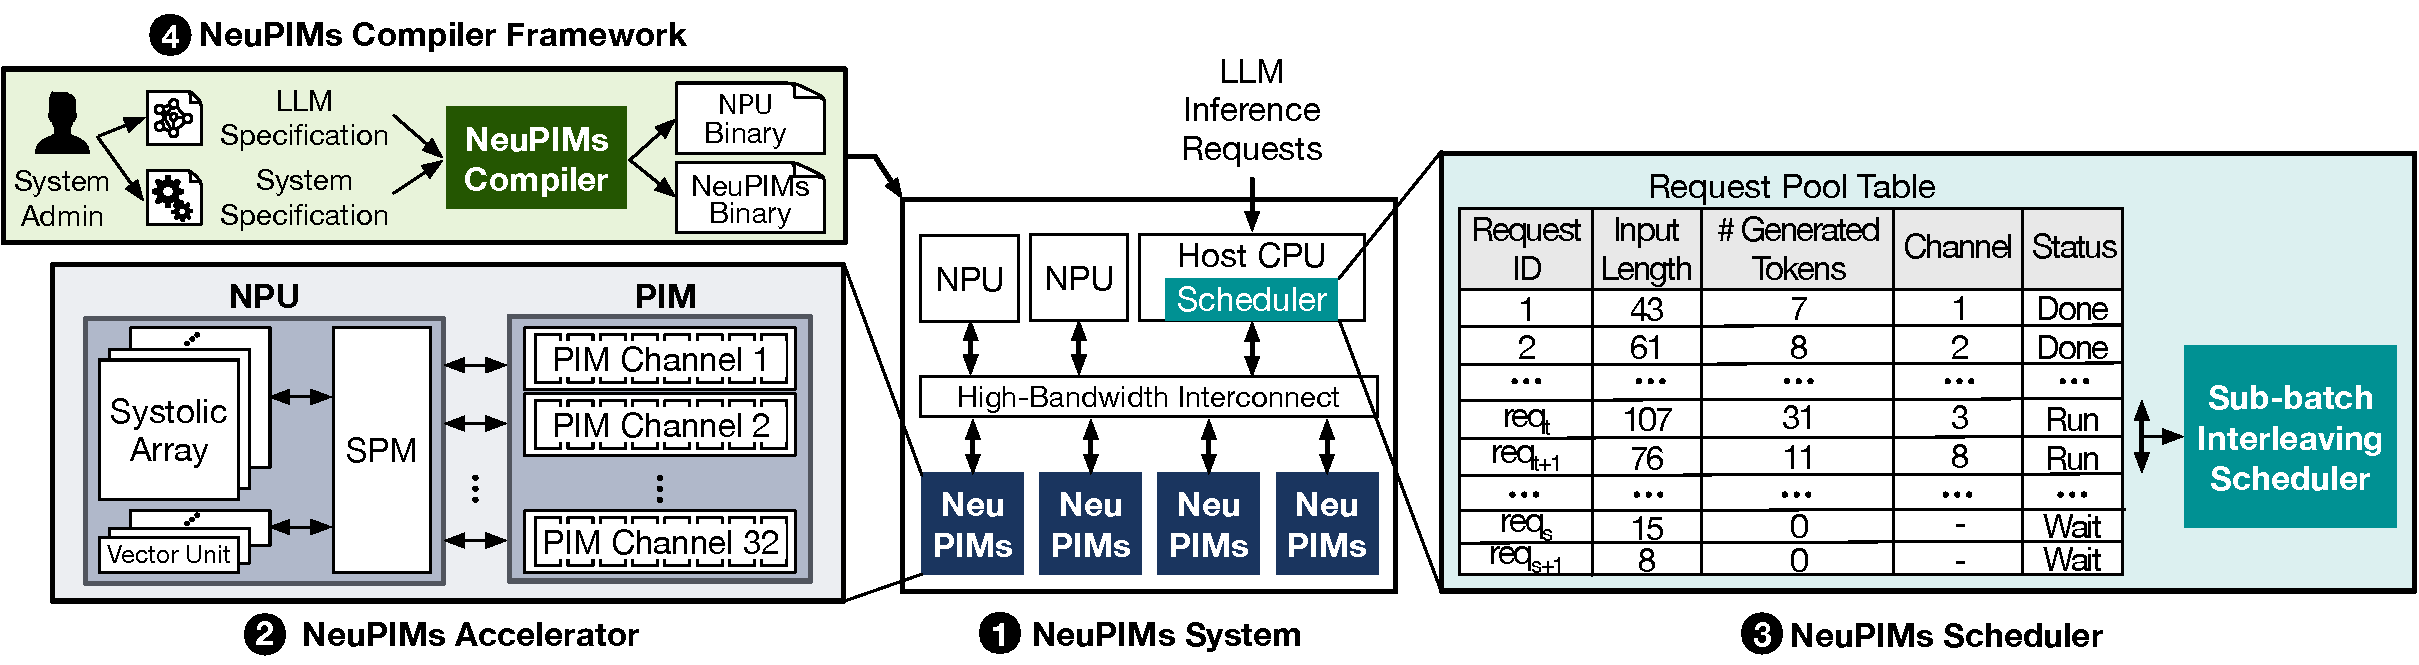
\includegraphics[width=1.0\textwidth]{figure/overview.pdf}
        \vspace{-3ex}
        \caption{Overview of the proposed \neupims system.}
        \vspace{-2.5ex}
        \label{fig:overview}
\end{figure*}

\subsection{A Na\"ive NPU-PIM Approach}

A straightforward approach to resolve this bandwidth bottleneck is to exploit the Processing-in-Memory (PIM) technology, which allows offloading the bandwidth-bound computations to its in-memory accelerator.
%
Thus, we design a na\"ively integrated NPU-PIM accelerator, exploiting a systolic array architecture for the NPU and incorporating a state-of-the-art PIM-based GEMV accelerator, Newton~\cite{newton}.
%
We use the same methodology as in Section~\ref{sec:gpu-analysis}, where we replace GPUs with a standard NPU-PIM integrated device. 
%
The detailed hardware and system simulation methodology are described in Section~\ref{sec:method}.
%
%
Figure~\ref{fig:npupim-utilization} presents the compute utilization of NPU and PIM for running different layers in the LLM decoder blocks.
%
The results show that while NPU is busy running QKV generation, projection, and FFN layers, PIM utilization stays at zero. 
%
On the other hand, NPU utilization becomes almost zero when PIM is running the MHA layers.
%
Consequently, the combined utilization of NPU and PIM, when measured across the entire execution time, is less than 40\% for both.
%


\niparagraph{Necessity of concurrent NPU and PIM executions.}
%
The observed under-utilization is primarily due to the fundamental limitation in PIM's microarchitecture that disallows the concurrent execution of host (NPU) and PIM units, which serializes the disjoint resource usages.  
%
Consequently, the most critical challenge in realizing the practical use of PIM in NPU accelerators is enabling their parallel executions. 
%
This research problem constitutes the focus of this work.